\documentclass{IEEEtran}

\usepackage[a4paper, top=3cm, left=2cm, right=2cm, bottom=2cm]{geometry}
\usepackage[ngerman]{babel}
\usepackage[utf8]{inputenc}
\usepackage[T1]{fontenc}
\usepackage{hyperref}
\usepackage{graphicx}
\usepackage{xcolor}

\graphicspath{ {./images/} }

\hypersetup{colorlinks=true, allcolors=black}

\title{Ansätze zum Echtzeit-Video-Streaming im Web}

\author{
	\IEEEauthorblockN{Maximilian Schulke \textit{(Matrikel-Nr. 20215853)}}\\
	\IEEEauthorblockA{
		Technische Hochschule Brandenburg \\
		B.Sc. Medieninformatik \\
		Computergrafik
	}
}


\begin{document}
\begin{onecolumn}

\IEEEspecialpapernotice{
	betreut durch Prof.\ Dr.\ rer.\ nat.\ Reiner Creutzburg\\
	Wintersemester 2021\\
	Abgabetermin \today
}

\maketitle

\begin{abstract}
	Das abstract schreibe ich zu letzt!
\end{abstract}

\tableofcontents

\listoffigures
\listoftables

\end{onecolumn}

\begin{twocolumn}
\markboth{Hausarbeit Computergrafik – Maximilian Schulke}{}

\section{Einleitung / Motivation}

\IEEEPARstart{M}{\MakeLowercase{it}} der zunehmenden Vernetzung der Arbeitswelt
in den letzten Jahren \textcolor{red}{quelle suchen corona zoom} werden auch
digitale Meeting-Systeme immer relevanter und müssen immer mehr Nutzer in
Echtzeit mit einander verbinden um einen reibungslosen Arbeitsalltag zu
gewährleisten. Dies impliziert natürlich auch dass eine \textcolor{red}{quelle
suchen ab wann gute Qualität} Verbindungsqualität gegeben sein muss, damit die
Systeme nutzbar bleiben.

\textcolor{red}{\& sicherheitsaspekt}
Aber wie können wir skalierbare Meeting-Systeme realisieren ohne große
Datenmengen über einen Streaming-Server zu schicken der diese an alle anderen
broadcasted? Die Entwicklung der letzten Jahre deuten immer mehr darauf hin,
dass \textit{Peer-To-Peer} basierte Lösungensansätze aufgrund der besseren
Performance und Skalierbarkeit, in der Regel die bessere Wahl darstellen
\textcolor{red}{quelle suchen}. Natürlich spielen zur Auswahl der Architektur
noch weitere Parameter eine wichtige Rolle (z. B. die maximale Bandbreite und
Rechenleistung der Endgeräte), aber mit immer großer werdenden
Heimnetz-Leitungen und zunehmender Rechenleistung der Endgeräte stellt dies
meistens kein Problem mehr da. \textcolor{red}{quelle suchen}.

Die Problematik der Echtzeit-Kommunikation im Web beschäftigt auch
das \textit{W3C} seit 2011 im Zuge der Standardisierung des seit diesem Jahr
zum Web-Standard erklärten Protokoll \textit{WebRTC}. \textcolor{red}{quelle
suchen}.

Es ist also (immer noch) eine sehr aktuelle Thematik in der Informatik
Echtzeit- oder \textcolor{blue}{Nahe-Zu-Echtzeit-Kommunikation} zuverlässig zu
bewältigen. Die Aufgabe dieser Arbeit soll sein, einen Überblick über den
Stand der Architekturmuster, Protokolle und möglicher Problematiken bei der
Implementierung von eigenen Echtzeit-Video-Streaming-Diensten geben,
\textcolor{orange}{diese anhand eines Experiments durchsprechen und auswerten
usw.}

\section{Historie der Echzeit-Übertragung}

Um zu verstehen wie sich die Protokolle hin zum heutigen Stand entwickelt
haben, ist es besonders interessant nachzuvollziehen wie die ersten Schritte
der IEFT oder auch \textit{Internet Engineering Task Force} bezüglich der
Echtzeit-Kommunikation aussahen, welche Probleme erkannt und behoben wurden und
welche Protokolle heute der Standard sind.

\subsection{1996: RTP \& RTCP – RFC 1889}

Am weitesten reicht das \textit{Real-Time Transport Protocol} oder auch
\textit{RTP} zurück. Es wurde erstmals 1996 von der IEFT standardisiert und
stellt seit dem einen Grundbaustein der datenformatsaganostischen
Echtzeit-Übertragung da. Es kann für diverse
Echtzeit-Übertragungs-Problematiken dienlich sein, da jegliche Binärdaten
verschickt werden können; Somit gibt es keinen ``Lock-In'' auf bestimmte Audio-
oder Video-Codecs. \textcolor{orange}{aussage prüfen und quelle}.

\textit{RTCP} ist das mit \textit{RTP} einhergehende Kontrollprotokoll. Es
wird primär dazu verwendet, die Übertragungsparameter der Sender zu
beeinflussen – z. B. durch ein Feedback zur Übertragungsqualität oder ein
Abmelden der Session. Desweiteren bietet es eine persistente ID für die
\textit{RTP}-Mitglieder, die über Programm-Neustarts hinweg zur Identifikation
von Mitgliedern und der zuordnung von Datenströmen verwendet werden können.
\textcolor{red}{cite rfc1889 kapitel 6 / 6.1 bzw. S. 15-17}

Das Protokoll siedelt sich im TCP/IP-Stack über \textit{UDP} an
\textcolor{red}{cite rfc1889 introduction}. Es fügt wichtige Informationen zu
UDP-Datagrammen hinzu: Im wesentlichen eine Sequenznummer um die
Sende-Reihenfolge zu codieren und einen Payload-Type, der den Codec des
Segments angibt. Somit kann auch bei nicht sequenziell übertragenden
Datagrammen die Ursprüngliche Reihenfolge rekonstruiert werden und es können
bei verlorenen Segmenten Interpolationsalgorithmen verwendet werden.
\textcolor{red}{quelle / beispiele suchen}. Der Payload-Type ist essenziell um
ohne Session-Aushandlung zu kommunizieren wie der Empfänger die Daten zu
decodieren hat, um eine Sinnvolle nachricht zu erhalten.

In der ersten Version aus 1996 gab es einige Probleme bezüglich
\textcolor{red}{Probleme suchen}. Diese wurden 2003 in dem RFC3550
überarbeitet - somit wurde das RFC1889 durch die neuere Version 3550 obsolet.
In der aktuelleren Version wurden einige Änderungen eingearbeit: Im
wesentlichen ``RTCP Packet Send and Receive Rules'' ``Layered Encodings''
``Congestion Control'' ``Security Considerations'' ``IANA Considerations''
\textcolor{orange}{Dummer text}.

Eine wichtige Voraussetzung zur Verwendung von \textit{RTP} ist ein externer
\textit{Signaling-Server}, den alle Beteiligten zur Session-Aushandlung
verwenden. Ein Standard hierfür ist im \textit{RTP-Framework} selbst nicht
definiert, eine beliebte Wahl für ein Protokoll zur Session-Aushandlung ist
allerdings das \textit{Session Initiation Protokoll} (oder kurz \textit(SIP)).
% https://datatracker.ietf.org/doc/html/rfc3550#section-3

\subsection{2004:\ SRTP (RFC 3711)}

Im März 2004 wurden \textit{SRTP} und \textit{SRTCP} vorgestellt – die
verschlüsselten Version von \textit{RTP} bzw. \textit{RTCP}. Diese bauen
weitestgehend auf dem \textit{Advanced Encryption Standard} (kurz.
\textit{AES}) auf \textcolor{red}{(siehe RFC3711 Seite 19).}. Der RFC
beschäftigt sich weitestgehend mit den kryptografischen Aspekten des
Protokolls.

Eine weitverbreitete und offene Implementierung für \textit{SRTP / SRTCP}
wird von der US-Amerikanischen Telekomunikations-Gesellschaft Cisco
bereitgestellt. Diese hat den Namen \textit{libsrtp} und ist öffentlich auf der
Entwickler-Plattform GitHub einsehbar (siehe
\href{https://github.com/cisco/libsrtp}{github.com/cisco/libsrtp}).

% Anwendung in VoIP\!
% https://de.wikipedia.org/wiki/ZRTP

\subsection{2005: RTMP von Adobe}

% https://www.adobe.com/content/dam/acom/en/devnet/rtmp/pdf/rtmp_specification_1.0.pdf
\textit{RTMP} ist ein von der Firma \textit{Adobe Systems Incorporated}
spezifiziertes Protokoll zur Echtzeit-Übertragung von Multimedia-Streams.
\textit{RTMP} wurde laut Spezifikation\textcolor{red}{siehe RTMP spec 1.0},
entwickelt um über dem Transport-Protokoll \textit{TCP} verwendet zu werden.

Das Protokoll wurde dazu entwickelt um im Kontext eines Flash-Players verwendet
zu werden. Dies führt dazu, dass es heutzutage nurnoch bedingt Anwendung
findet, da mittlerweile viele Browser ihren Flash-Player-Support eingestellt
haben (\textcolor{red}{siehe Chrome und Firefox}) % https://support.mozilla.org/en-US/kb/end-support-adobe-flash

Außerdem spricht die hohe Latenz von bis zu 30 Sekunden, die durch die
Verwendung von \textit{TCP} zustandekommt (\textcolor{red}{siehe
restram.io/streaming-protocls}), gegen den Einsatz von \textit{RTMP} in einem
Echtzeit-Übertragungs-Kontext.

Desweiteren gibt es noch Protokollvarianten die HTTP bzw. HTTPS als zugrundeliegendes
Protokoll verwenden.\textcolor{red}{Siehe XYZ Quelle suchen}

\subsection{2010: WebRTC (RFC 8825)}

\textit{WebRTC} ist eine Peer-To-Peer-Technologie die über mehrere Protokolle
und Audio- und Video-Codecs performante und generische
Echtzeit-Kommunikations-Kanäle zwischen Nutzern (oder auch \textit{Peers})
realisiert. Sie 

WebRTC stellt eine direkte Verbindung zwischen zwei Endgeräten her und
verwendet einen mix aus RTP, RTCP, SDP, (ICE Candidates) und einem signaling
server. Es unterstützt beliebte video codecs wie V8 / V9 und ist in der zukunft 
auf AV1 angelegt. Der standard audio codec ist opus.

Durch die direkte verbindung wird eine sogennante sub second latency erreicht.
Dies beschreibt im grunde \textcolor{red}{XYZ}.

% Hat mit 1996 RTP und dann 2005 mit RTMP angefangen, wann kam SRTP?\ JSEP Global IP Solutions \& Google WebRTC kam 2010, Microsoft wollte CU-RTC

% > Datenströme sind verpflichtend zu verschlüsseln. Dazu werden Verbindungen über DTLS verschlüsselt und Audio- und Videokommunikation zusätzlich durch SRTP geschützt.[16]
% https://datatracker.ietf.org/doc/html/rfc8834#section-4.1

% https://www.w3.org/2021/01/pressrelease-webrtc-rec.html.en


Die ersten \textit{Requests for Comments} oder auch \textit{RFC} zu
den grundlegenden Protokollen \textit{RTP} und
\textit{\textcolor{blue}{Protokoll X}}, auf denen die heutigen Protokolle
weitestgehend aufbauen, wurden bereits in den späten 1990er Jahren
veröffentlicht und seit dem immer weiterentwickelt. \textcolor{red}{quelle
anhängen RFC35XX}.

\section{Architekturmuster}

In diesem Kapitel werden zwei der bekanntesten Architekturmuster in der
Echtzeit-Übertragung vorgestellt und verglichen. Es geht primär um die
verteilte Peer-To-Peer Architektur und die zentralisierte Relay / Broadcast
Architektur.

\subsection{Peer-To-Peer}

Auf Grund der hohen Anforderungen an möglichst niedrige Übertragungslatenzen
bietet eine Peer-To-Peer-Architektur klare Vorteile durch den stark verkürzten
Weg, den die Pakete zurücklegen müssen bis sie bei dem Empfänger ankommen.

Deutlich komplizierter wird allerdings die aushandlung bzw.\ initialisierung
einer Verbindung zwischen zwei peers, da diese sich nicht wie bei der typischen
client-server-architektur eine fixe adresse zur verbindung haben. Dieses
problem wird typischerweise über einen signaling server gelöst.

\subsubsection{Signaling Server}
Ein signaling server ist allen peers bekannt und dient als
kommunikationsplattform, damit sich die beiden (sich gegenseitig initial
unbekannten) peers gegenseitig vorstellen können.

Signaling server sind interessanterweise keine feste anforderung für peer to
peer muster. Wenn alle peers immer statische addressen hätten, könnten sie auch
offline ihre ips / ice candidates / sdp offers etc.\ austauschen und so eine
session aufbauen. Wichtig ist leidlgich eine initiale out of band
kommunikation.

Der signaling server kann außerdem noch nach verbindungsaufbau dazu verwendet
werden um die bestehende verbindung zu optimieren. Peers können neue ICE
candidates vorschlagen um die Übertragung an neue gegebenheiten im internet
(z.B. ausfall eines routers) anzupassen. (siehe mdn)

% https://datatracker.ietf.org/wg/wish/about/

\subsubsection{Holepunching}
Holepunching beschreibt den prozess lokale firewalls und nats zu durchbrechen
um eine direkte verbindung zwischen zwei endgeräten herzustellen.

% https://datatracker.ietf.org/doc/html/rfc8834#section-10
% https://de.wikipedia.org/wiki/Multicast
% peer to peer wäre möglich mit ip multicast mit vielen usern ohne pakete zu
% duplizieren

\subsubsection{IP-Multicast}

Je mehr Nutzer / Endgeräte an einer peer-to-peer-übertragung teilnehmen, desto
größer wird die Belastung der Bandbreite bei den einzelnen Teilnehmern. Jedes
Paket muss nicht einmal, sondern n-mal verschickt werden (wobei n die anzahl
der teilnehmer ist). Dies kann bei labilen oder einfach schwachen Netzwerken
entweder zur verminderung der übertragungsqualität führen, oder in besonders
schlimmen fällen sogar das restliche netzwerk eines einzelnen Teilnehmers
negativ beeinflussen, da dieser die meiste Bandbreite für die wiederholte
übertragung gleicher pakete verwendet.

Eine theoretische Lösung für dieses Problem, ist die Verwendung von
IP-Multicast-Adressen. Diese erlauben es einem Gerät ein IP-Paket einmalig zu
übertragen, und dieses von Multicast-Routern im internet multiplizieren zu
lassen. (Siehe grafik)

Vergleichs grafik einfügen..

Dieser ansatz hat klare vorteile: Das gesamte - lokale \& globale – netzwerk
wird geschont. So würde die Anzahl möglicher Teilnehmer deutlich steigen, da
ein Netzwerk-Bottleneck erst bei einem zu großen Download-Volumen des
empfangenen Contents eintreten würde.

\subsection{Relay}
% https://webrtc.org/getting-started/turn-server

\section{Protokolle}
\subsection{RTP}

\subsection{RTCP}
\subsection{RTSP}
\subsection{SDP}
% https://datatracker.ietf.org/doc/html/rfc4566#section-3.1
\subsection{SID}
% https://datatracker.ietf.org/doc/html/rfc3261
% \subsection{STUN}
\subsection{WebRTC}

\section{Implementierung eines Kamera-Live-Streams}

In diesem Kapitel wird ein experimentelles Kamera-System entwickelt, das die
oben erläuterten Protokolle / Technologien verwendet.

\subsection{Ziel}
Ziel dieses Experiments ist es eine möglichst einfach ein funktionierendes
System zu entwickeln und mögliche Probleme, benötigten Zeitaufwand usw.\ zu
ermitteln.  Desweiteren ist ein ``Performance'' Vergleich mit anderen
Live-Stream systemen interessant. Es gilt also die frage zu klären, wie viel
arbeit benötigt ein grundsätzlich funktionierendes Software-Produkt das auf
Echtzeit-Übertragung beruht.

\subsection{Umfang}

Das zu implementierende Kamera-System wird lediglich eine einzige Kernfunktion
aufweisen: Sobald die Kamera an ist, streamt sie via WebRTC, mit ausreichend
FPS (mindestens 15 im durchschnitt) in ausreichender Qualität (720 x\ 480),
ihre Aufnahmen an ein User Interface. Dieses wird im Browser laufen, muss aber
ausreichend Alternativen für andere Plattformen aufweisen (Nativ, Smartphone
usw.). Das Interface und die Kamera starten die Aushandlung des
WebRTC-Streams über den Signaling Server. D.h.\ sie versenden SDP (Offer /
Answer) und tauschen ihre ICE-Candidates aus.

\subsection{Architektur}

\begin{figure}[ht]
	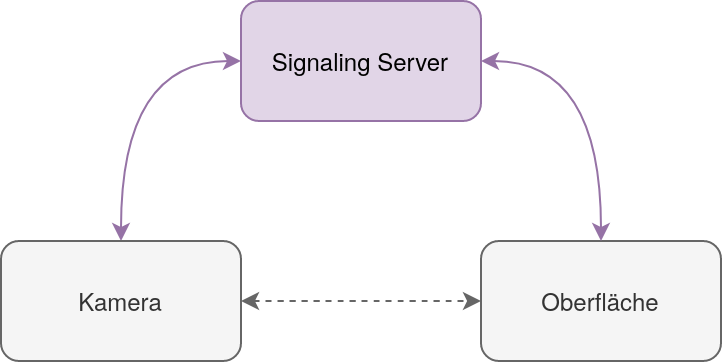
\includegraphics[width=0.5\textwidth]{diagram-signaling}
	\centering
	\caption{Signaling zwischen der Kamera und dem Interface (Angelehnt an IEEE
	PAPER!!!!!!!!!!!)}
\end{figure}

Die angedachte Architektur wurde möglichst einfach gehalten. Sie besteht
lediglich aus 3 Elementen:

\subsubsection{Kamera}

Für dieses Experiment wurde ein Einplatinencomputer der Marke Raspberry PI in
der 4. Version mit 8GB RAM – erweitert durch ein Drittanbieter-Kamera-Modul –
verwendet. Dieser ist allerdings absolut austauschbar, da jeder Rechner der
die u.g. Hauptanforderung erfüllt eine geeignete Umgebung darstellt – so kann
die Kamera-Software auch auf einem Laptop ausgeführt werden, falls keine
Hardware verfügbar ist. Dies wurde zur veranschaulichung mit einem ThinkPad
T490 und einer aktuellen NixOS Installation getestet.

Die Hauptanforderung an die Hardware auf der die Kamera-Software läuft ist eine
Linux-Installation (mit den entsprechenden installierten Paketen für die
Abhangigkeiten) und eine angeschlossene Kamera die von Linux erkannt wird.

Auf der Einplatinencomputer ist das mitgelieferte Betriebssystem ``Raspberry PI
OS'' und die entsprechenden Software-Abhängigkeiten installiert. 
\textcolor{red}{Siehe GitHub für Dependencies.}

\subsubsection{Signaling-Server}

Der Signaling-Server ist ein WebSocket-Secure-Server, der zwei
WebSocket-Verbindungen miteinander verknüpft. Er verwaltet sogenannte Räume.
Ein Raum besteht aus 0 bis 2 Clients und dient dazu diese miteinander zu
verbinden. Auf dem Server kann es mehrere Räume gleichzeitig geben – dadurch
könnte dieser Signaling-Server theoretisch auch noch für weitere
WebRTC-Anwendungen verwendet werden. Ein Raum hat eine ID, diese ist eine
256-Bit-Entropie. Clients werden durch eine 128-Bit-Entropie identifiziert.

So können sich zwei Clients durch ein Out-Of-Band kommuniziertes Secret (die
Raum-ID) über diesen in Kontakt treten. Diese könnte beispielsweise, würde es
sich bei der entwickelten Kamera um ein echtes Produkt handeln, bei der
Herstellung generiert werden, ausgedruckt und neben die Kamera in die
Verpackung gelegt werden.

\subsubsection{Interface}

Das Interface verbindet sich mit dem Signaling Server und nimmt eine Raum-ID
entgegen. Mit dieser Raum-ID wird dann auf dem Signaling Server entweder ein
neuer Raum erstellt, falls noch keiner mit der ID existiert, oder es wird dem
bestehenden Raum beigetreten. Nach dem ein weiterer User beigetreten ist, fängt
der in \textcolor{red}{Kapitel XY} erklärte Aufbau eines WebRTC-Streams zu dem
Nutzer an.

\subsection{Signaling Server}

Als erstes wurde der Signaling Server entwickelt, da dieser keine
Abhängigkeiten an seine Clients hat. Die Kamera-Software und Interface setzen
beide jeweils den laufenden Signaling Server vorraus um korrekt zu
funktioneren.

\subsubsection*{Asynchronität}

Eine logische Anforderungen an den Server ist das gleichzeitige verarbeiten
mehrerer Verbindungen – ansonsten könnte immer nur ein Client alleine mit dem
Server Verbunden sein. Dies würde die Signaling-Funktionalität eines Raumes
unbrauchbar machen.

Die asynchrone Programmierung ist ein Konzept zur Lösung dieser Problemklasse.
Da langlebige Verbindungen in der Regel einen großteil der Zeit ungenutzt sind,
ist es naheliegend Verbindungen ohne neue Ereignisse keine CPU-Zeit zu geben
um andere Verbindungen in der Zeit abzuarbeiten, in der auf Ereignisse gewartet
wird.

HIER ZIETIEREN WAS DAS ZEUG HÄLT / ERKLÄRGRAFIKEN NUTZEN

\begin{figure}[ht]
	\includegraphics[width=0.5\textwidth]{diagram-asynchronität}
	\centering
	\caption{Asynchrone Abarbeitung einer IO intensiven Aufgabe}
\end{figure}

\subsubsection{Verbindungsaufbau}

\begin{figure}[ht]
	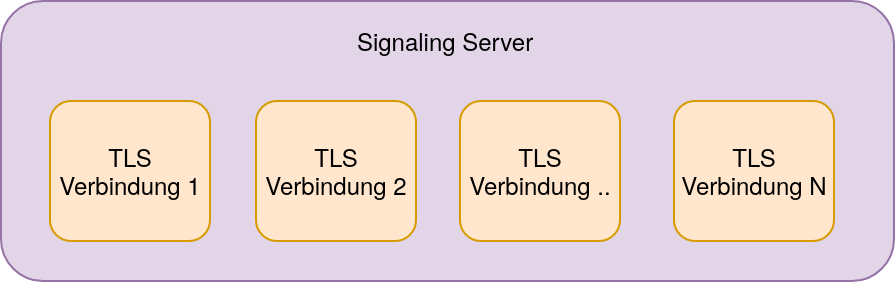
\includegraphics[width=0.5\textwidth]{diagram-signaling-server-tls}
	\centering
	\caption{Signaling-Server mit mehreren TLS Verbindungen}
\end{figure}


Um eine WebSocket-Secure-Verbindung aufzubauen, muss zu erst eine TCP- und dann
darüber eine TLS-Verbindung zu dem Client aufgebaut werden. Über diese wird
dann zu erst in HTTP kommuniziert (siehe WebSocket verbindungsaufbau Quelle
suchen) und nach einer erfolgreichen Nachricht des Servers mit dem Status-Code
101 (Switching Protocols) wird die über den gleichen Transport-Weg (TLS)
nach dem WebSocket-Protokoll kommuniziert.

\textcolor{red}{Grafik einfügen}

\subsubsection{Spezifikation des Signaling-Protokolls}

Das Signaling-Protokoll ist in 2 Nachrichten-Typen unterteilt:
Server-Nachrichten und Peer-Nachrichten. Clients dürfen nur Peer-Nachrichten
senden, ansonsten wird die Verbindung aufgrund eines Protokoll-Verstoßes
geschlossen. Der Server verschickt nur Server-Nachrichten.

Alle Protokoll-Nachrichten werden in JSON kodiert und dann über den
WebSocket-Nachrichten-Typ Binär an den Empfänger geschickt werden.

\vspace{0.5em}

\textbf{Server-Nachrichten}

\begin{itemize}
	\item Hello \{Client-ID\}
	\item Joined
	\item Error
	\item Room/Join \{Client-ID\}
	\item Room/Leave \{Client-ID\}
	\item Room/Signal \{Signal\}
\end{itemize}

\vspace{0.5em}

\textbf{Peer-Nachrichten}

\begin{itemize}
	\item JoinOrCreate \{Raum-ID\}
	\item Signal \{Signal\}
\end{itemize}

\vspace{0.5em}

Nach einer erfolgreich aufgebauten Verbindung mit dem Server schickt dieser ein
\textit{Hello} mit der zugewiesenen Client-ID.\ Darauf hin muss der Client ein
\textit{JoinOrCreate} senden um einem Raum beizutreten. Bevor der Client die
Nachricht \textit{Joined} vom Server erhält, darf dieser keine Signale
verschicken.

\textcolor{red}{Diagramme einfügen!}

Eine \textit{Room/Join} Nachricht wird an ggf.\ andere Clients im Raum
verschickt, sobald ein Client diesen betritt. Diese Nachricht kann auf dem
Client als anlass genutzt werden eine SDP-Offer zu erstellen, da nun sicher
ist, das ein anderer Client im Raum ist. Wenn beide Clients sich an dieses
Schema halten, schickt immer der Client, der sich zu erst Verbunden hat die
Einladung und der andere die Answer.

Analog wird eine \textit{Room/Leave} Nachricht verschickt wenn ein Client einen
Raum verlässt.

Die \textit{Room/Signal} Nachricht wird an den Empfänger eines Signals
geschickt, nachdem der Sender des Signals eine \textit{Signal} Nachricht an den
Server geschickt hat.

\subsubsection{Raum-Verwaltung}

Die Raum-Verwaltung fällt unter anderem in die Kategorie der
Synchronisationsprobleme. Es gibt unter Umständen $n$ Client-Verbindungen, die
den Status von einem Raum erfragen wollen, und ggf.\ einen Anlegen möchten. Dies
soll für alle Verbindungen öffentlich geschehen, Clients dürfen sich aber dabei
nicht gegenseitig überschreiben.

% Mutual exclusion -> gegenseitiger ausschluss -> nur einer darf

Um zwei asynchron laufende Programmteile zum sequenziellen Zugriff auf
gemeinsamen Speicher zu zwingen, gibt es Möglichkeit einen Semaphor bzw. Mutex
zu verwenden. Dieser blockiert den Teil des Programms, der gerade auf den
gemeinsamen Speicher zugreifen möchte solange, bis ein ggf.\ anderer Zugriff
beendet ist. Um Deadlocks bzw. Inperformante Code-Abschnitte zu vermeiden, ist
es ratsam einen Mutex nicht über länger andauernde Operationen hinweg zu
locken, da sonst für diese Zeit alle anderen Teile des Programms, die gerade
auf den Speicher zugreifen möchten blockiert sind.

Als konkrete Lösung für das bestehende Problem bietet sich eine HashMap, deren
zugriff von einem Mutex kontrolliert wird, an. Jede Client-Verbindung, die
aktuelle Raum-Informationen braucht (was hauptsächlich bei dem erstellen /
betreten von Räumen der Fall ist), muss nun vorher erst den mutex locken. 

\subsubsection{Kommunikation zwischen mehreren Client-Verbindungen}

Bis zu diesem Punkt ist der Aufbau der Verbindung und das zu implementierende
Protokoll klar, allerdings fehlt noch das Verknüpfen von Client-Verbindungen um
Signale weiterzuleiten.

Da bereits Räume verwaltet werden, liegt es nahe dort einen Kommunikationskanal
einzubetten. Eine Implementierung für diesen Kommunikationskanal stellen z.B.
sogenannte Channels dar. Diese erlauben Inter-Thread- (und im asynchronen
Kontext: Inter-Task-) Kommunikation über ein einfaches
Sender-Empfänger-Prinzip. Ein Channel ist unterteilt in eben diese beiden
Teile: Der Sender darf Nachrichten schreiben, der Empfänger darf sie aus dem
Channel lesen.

In diesem Fall ist allerdings zusätzlich noch bidirektionale Kommunikation
gefragt, da beide Clients Signals des jeweils anderen erhalten sollen. Dafür
bieten sich sogenannte Broadcast-Channel an. Sie sind dafür ausgelegt, dass von
mehreren Stellen in diese geschrieben und gelesen wird. Sie funktioneren analog
zu dem Broadcast aus der Netzwerktechnik.

Diagramm einfügen..

%      C
%    s r r
%  s   r   r
% o    o     o

%      C
%    r s r
%  r   s   r
% o    o     o

%      C
%    r r s
%  r   r   s
% o    o     o

\begin{figure}[ht]
	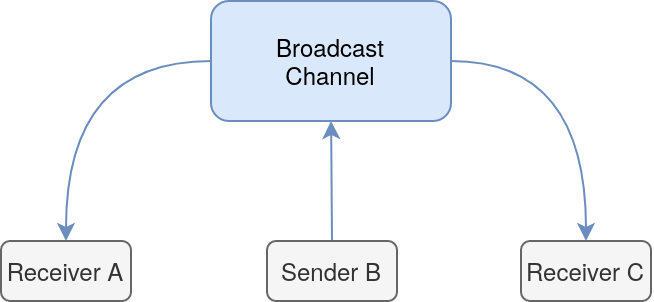
\includegraphics[width=0.5\textwidth]{diagram-broadcast}
	\centering
	\caption{Broadcast-Channel Konzept}
\end{figure}

Somit kriegt jeder Client bei betreten eines Raumes Zugriff auf einen Sender
und einen Empfänger dieses Broadcast-Channels. In diesen schreibt er bei erhalt
einer Peer-Nachricht vom Typ \textit{Signal} das Signal. Eine Client-Verbindung
die gerade keine CPU-Zeit erhält, da ansonsten keine Ereignisse aufgetreten
sind, wird wieder aktiv sobald eine neue Nachricht über den Channel da ist.
Diese kann dann als Server-Nachricht vom Typ \textit{Room/Signal} mit dem
Signal aus dem Channel an den Empfänger gesendet werden.

\begin{figure}[ht]
	\includegraphics[width=0.5\textwidth]{diagram-websocket-verknüpfung}
	\centering
	\caption{Kommunikation von Nutzern über einen Broadcast-Channel}
\end{figure}

\subsection{Interface}

Um den Signaling-Server für ein erstes nutzbares Zwischenergebnis zu verwenden,
wurde eine einfache browserbasierte Benutzer-Oberfläche implementiert, die
analog zu sehr bekannten Videokonferenz-Systemen wie z.B. Zoom oder Google Meet
funktioniert. Bei diesem Experiment wurde der Fokus primär auf die
Bildübertragung gelegt – eine Audioübertragung könnte aber ohne großen Aufwand
implementiert werden.

Ein Benutzer muss über dieses Interface einem beliebigen Raum auf dem
Signaling-Server beitreten können. Sobald ein weiterer Benutzer beitritt soll
der erste eine Nachricht erhalten, dass Jemand seinem Raum beigetreten ist.
Letztendlich soll die Aushandlung der Video-Übertragung zwischen den beiden
Benutzern ohne weitere Interaktion des Benutzers stattfinden.

\subsubsection{WebSocket-Verbindung}

Als Vorkehrungen für die singalisierungs Kommunikation mit dem Signaling-Server
muss eine WebSocket-Secure Verbindung mit dem Server aufgebaut werden. Dies
gelingt ebenfalls über eine Web-API:\
https://developer.mozilla.org/de/docs/Web/API/WebSocket

Nun meldet sich der Server nach dem Verbindungsaufbau als erstes mit der
\textit{Hello}-Nachricht und weist uns eine ID zu. Nach dieser ersten Nachricht
können wir die eigentliche Anwendung starten.

\subsubsection{Erstellen / Beitritt eines Raumes}

Um festzustellen mit wem sich der Benutzer verbinden möchte, muss dieser
eine Raum-Id angeben. Diese ist als 64 Zeichen langen Hex-String einzugeben.

Nach erfolgreicher Eingabe einer Raum-Id wird diese mit der Nachricht
\textit{JoinOrCreate} an den Server geschickt, dieser verarbeitet die Anfrage
und schickt dem Benutzer eine \textit{Joined}-Nachricht. Ab diesem Zeitpunkt
wird eine \textit{RTCPeerConnection} erstellt, da ggf.\ bereits ein anderer
Nutzer im Raum war, der dem neu dazugekommenen eine SDP-Offer schicken wird.
Um diese Zeitnah zu verarbeiten, findet die Initialisierung vor der ersten
Signalisierungs-Nachricht statt.

% https://webrtc.org/getting-started/media-devices

\subsubsection{Verbindungsaufbau}\label{browser-webrtc}

Moderne Browser wie Firefox, Chrome, Safari etc.\ stellen eine Implementierung
des WebRTC-Stacks bereit, die durch eine übersichtliche API leicht zu
integrieren ist. % Siehe https://caniuse.com/?search=webrtc

Um eine vollständige WebRTC-Verbindung aufzubauen ist bei beiden Nutzern eine
RTCPeerConnection aufzubauen. Auf einer RTCPeerConnection ist eine
Event-basierte API verfügbar. (Siehe tabelle)

% table mit der API und der quelle der API:

Insbesondere sind für den Verbindungsaufbau die Events onnegotiationneeded und
onicecandidate von Interesse. Sobald eine Verbindung erstellt wurde und ein
lokaler Stream zu dieser hinzugefügt wurde, wird das onnegotiationneeded Event
ausgelöst. An diesem Punkt ist nun eine eigene SDP-Offer zu erstellen und über
den singalisierungs Server an den Empfänger zu versenden. Der Empfänger
verarbeitet diese anschließend und antwortet mit einer SDP-Answer. Nach dem
beide Teilnehmer die SDP-Nachrichten füe ihren Kommunikationspartner und sich
selbst gesetzt haben (siehe setRemoteDescription und setLocalDescription),
werden vom Browser onicecandidate-Events ausgelöst um eine direkte Verbindung
zwischen den beiden Browsern auszuhandeln.

% Signalisierungsablauf zwischen Interface und Kamera visualisiert:

\begin{figure}[ht]
	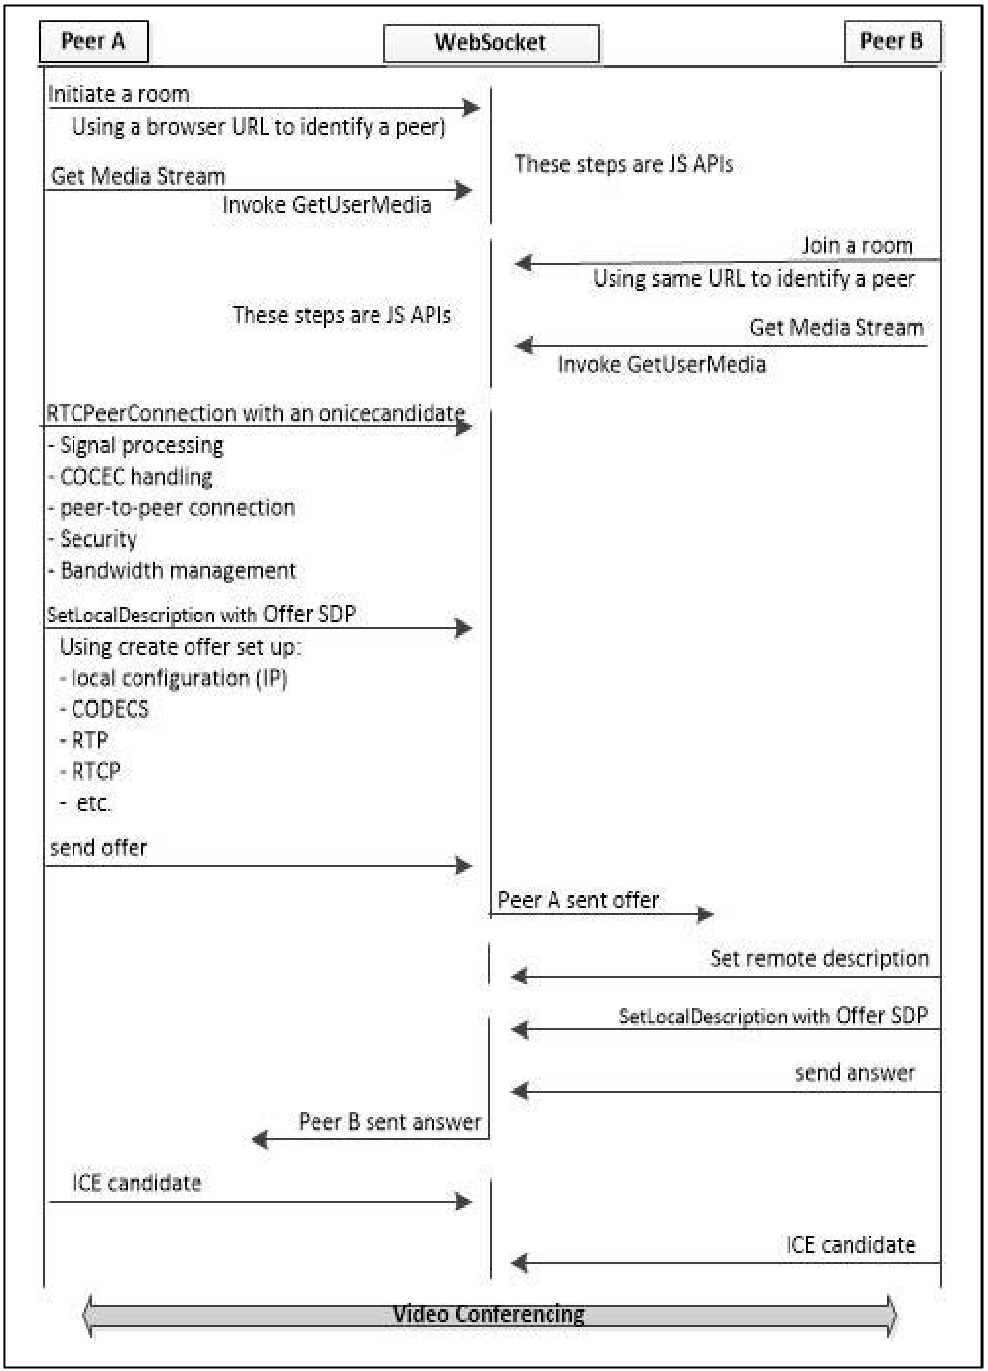
\includegraphics[width=0.5\textwidth]{cited-webrtc-connection-establishment}
	\centering
	\caption{WebRTC-Verbindungsaufbau (Siehe QUELLE)}
\end{figure}


Nach einem leeren ICE-Kandidaten ist die aushandlung abgeschlossen und der
Stream kann nun konsumiert werden.

\subsubsection{Verbindungsabbau}

Nach dem der Signalisierungs-Server eine \textit{Room/Leave}-Nachricht gesendet
hat, kann die RTCPeerConnection ohne negative Auswirkungen abgebaut werden. Im
Interface wird die Anzeige des Video-Streams des anderen Teilnehmers
zurückgesetzt und die RTCPeerConnection geschlossen. Somit ist das Interface
wieder bereit einem weiteren Raum beizutreten und erneut eine WebRTC Verbindung
herzustellen.

% Screenshots des Demos Interfaces anfügen

\subsection{Kamera}

Zu letzt ist die Kamera zu entwickeln..

\subsubsection{GStreamer}

Anders als in einer Browser-Umgebung bietet Linux abgesehen von
Hardware-Treibern keine wirklichen Abstraktionen für die Verwendung einer
Kamera und automatischer Bildverarbeitung. Dies ist in einer nativen Umgebung
die Aufgabe von weiteren Programmen und Bibliotheken.

Hier wird das weitverbreitete Multimedia-Framework GStreamer relevant. Dieses
abstrahiert sämtliche Zugriffe auf medienbezogene Hardware (in diesem Fall die
Kamera), beherscht die meistgenutzten Media-Codecs für Audio und Video und kann
über Plugins mit weiteren Funktionalitäten erweitert werden: Wie zum Beispiel
WebRTC.\

Somit muss die folgende Liste an Abhängigkeiten installiert werden, damit die
Kamera-Software korrekt funktioniert:

\begin{itemize}
	\item libgstreamer1.0dev oder so..
	\item Paketnamen raussuchen!!!
\end{itemize}

(Aufgelistet in Debian-Paket-Namen, da Raspberry PI Os Debian basiert ist)

GStreamer ist um das Konzept von Pipelines herum aufgebaut: Es 

\subsubsection{Architektur der Kamera-Software}

Die Kamera-Software ist grundsätzlich in 2 Schritte unterteilt, die endlos
wiederholt werden:

\begin{enumerate}
	\item Verbindungsaufbau zum Signalisierungsserver
	\item Verbindungsaufbau via WebRTC
\end{enumerate}

Im Regelfall dauert der 1. Schritt einige Millisekunden. Nach dem die
Verbindung zum Signalisierungsserver korrekt aufgebaut wurde (und die Kamera
dem festgelegten Raum beitreten konnte) wird eine GStreamer-Pipeline
initialisiert und auf den Beitritt eines Benutzers in den Raum erwartet. Nach
dem die \textit{Room/Join}-Nachricht eingetroffen wird die Pipeline auf Playing
gesetzt.

GStreamer unterstützt nach erfolgreicher Installation oben genannter Plugins
eine kompatible API zu der der Browser. Somit läuft der gesamte
WebRTC-Spezifische Verbindungsaufbau nach der exakt gleichen Logik ab wie unter
\nameref{browser-webrtc} erläutert.


\subsubsection{}

\subsubsection{Installation des Betriebssystems}

\subsubsection{Automatischer Start der Software}


\section{Benchmarks}

- CPU Load
- Netzwerkauslastung

\section{Auswertung}

- Raspberry Pi Kamera langsam..\ unerwünschte Qualität (evtl 32 bit?)

\section{Nächste Schritte}

\large{IPV6 only => NAT holepunching entfällt}

\section{Abbildungsverzeichnis}
abc
def

\bibliographystyle{IEEEtran}
\bibliography{IEEEabrv,references}

\newpage

\begin{appendix}

foo

\end{appendix}

\end{document}
